\documentclass[10pt,a4paper]{article}
\usepackage[utf8]{inputenc}
\usepackage{ae}
\usepackage[brazil]{babel}
\usepackage[vmargin=2cm,hmargin=2cm,columnsep=0.75cm]{geometry}
\usepackage{float,nonfloat}
\usepackage{graphicx,color}
\usepackage{subcaption}
\usepackage{amsmath}
\usepackage{verbatim}

\makeatletter
\let\@institution\empty
\def\institution#1{\def\@institution{#1}}
\renewcommand{\maketitle}{
    \begin{center}
        {\Large\bfseries\@title\par\medskip}
        {\large
            \begin{tabular}[t]{c}%
                \@author
        \end{tabular}\par\medskip}
        {\itshape\@institution\par}
        {\itshape\@date\par}
\end{center}}
\makeatother

\newcommand{\pixel}{\textit{pixel} }
\newcommand{\pixels}{\textit{pixels} }
\newcommand{\kernel}{\textit{kernel} }
\newcommand{\kernels}{\textit{kernels} }

\begin{document}
% ============================================================================

\title{MC920: Introdução ao Processamento de Imagem Digital\\Tarefa 7}
\author{
    \begin{minipage}{6cm}
        \centering
        Martin Ichilevici de Oliveira\\
        RA 118077
    \end{minipage}
    \and
    \begin{minipage}{6cm}
        \centering
        Rafael Almeida Erthal Hermano\\
        RA 121286
    \end{minipage}
}
\institution{Instituto de Computação, Universidade Estadual de Campinas}
\date{\today}

\maketitle

% ============================================================================

\section{Difusão anisotrópica}
A difusão anisotrópica consegue preservar as bordas da imagem durante um processo de remoção de ruídos através de blur.
Para preservar as bordas, a difusão anisotrópica utiliza conceitos de fluxo de calor e espaço escala. O espaço escala consiste em multiplas representações de uma imagem, aonde essas representações variam de altas resoluções à baixas resoluções.
Para construir o espaço escala, para cada nível $\sigma$ podemos fazer a convolução da imagem no nível zero(de maior resolução) com uma gaussiana, sendo representada como:

\begin{equation}
  I_{x,y}(\sigma) = I_{x,y}(0) * g(x,y,\sigma)
  \label{eq:escale_space}
\end{equation}

A equação de calor:

\begin{equation}
  \frac{\partial I}{\partial t} = \bigtriangleup I_{x,y}(t)
  \label{eq:heat_flow}
\end{equation}

Aplicada de forma discreta na difusão anisotrópica, resulta na seguinte equação:

\begin{equation}
  \frac{\partial I}{\partial t} = I(t + 1) - I(t) = \bigtriangledown \cdot (c_{x,y} \bigtriangledown I_{x,y}(t))
  \label{eq:time_step}
\end{equation}

Utilizando a máscara do Laplaciano:

\begin{equation}
  \left[\begin{array}{ccc}
    0 & +1 & 0\\
    +1 & -4 & +1\\
    0 & +1 & 0
  \end{array}\right]
  \label{mask:aniso_diff}
\end{equation}

Podemos expandir a equação \ref{eq:time_step} para:

\begin{equation}
  I(t + 1) = I(t) + \lambda (e^{\frac{-\bigtriangledown_N(i)^2}{k^2}} + e^{\frac{-\bigtriangledown_S(i)^2}{k^2}} + e^{\frac{-\bigtriangledown_W(i)^2}{k^2}} + e^{\frac{-\bigtriangledown_E(i)^2}{k^2}})
  \label{eq:time_step}
\end{equation} 

Aplicando-se esta máscara, obtemos bons resultados, como ilustrado na Figura \ref{fig:aniso_diff_ex}.

\begin{figure}[!ht]
    \centering
    \begin{subfigure}[ht]{0.45\textwidth}
        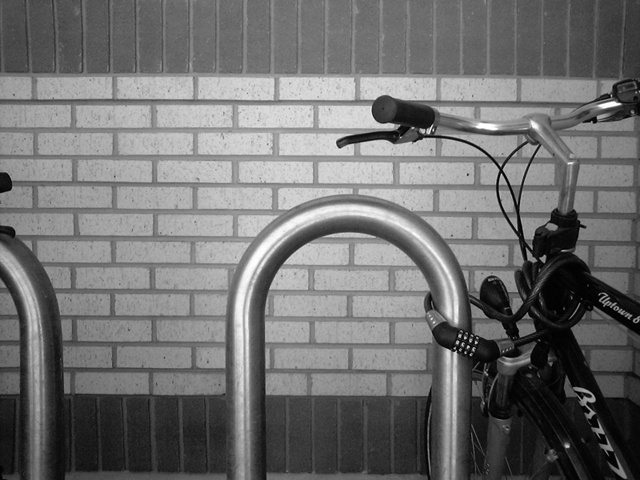
\includegraphics[width=\textwidth]{src.jpg}
        \caption{Figura original\cite{bike}}
        \label{fig:src}
    \end{subfigure}
    \qquad
    \begin{subfigure}[ht]{0.45\textwidth}
        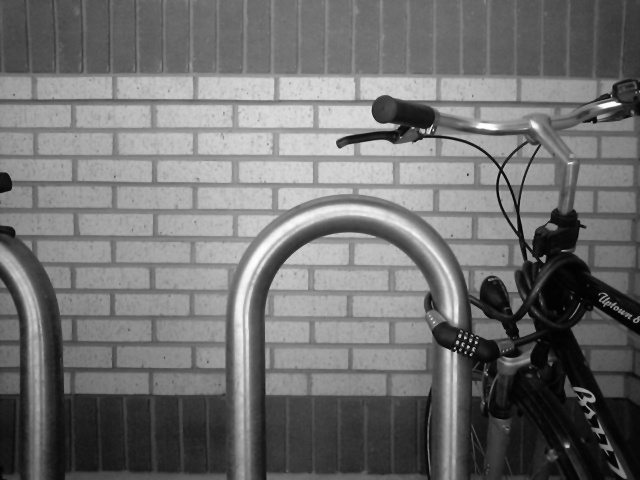
\includegraphics[width=\textwidth]{aniso.jpg}
        \caption{\centering Após aplicação de difusão anisotrópica}
        \label{fig:aniso_diff}
    \end{subfigure}
    \caption{Imagem original e com difusão anisotrópica}
    \label{fig:aniso_diff_ex}
\end{figure}

\section{Testando com alguns ruídos}
\subsection{Sal e pimenta}
Adicionando ruído do tipo sal e pimenta à imagem, obtemos o resultado expresso na Figura \ref{fig:aniso_diff_sp}.
\begin{figure}[!ht]
    \centering
    \begin{subfigure}[ht]{0.4\textwidth}
        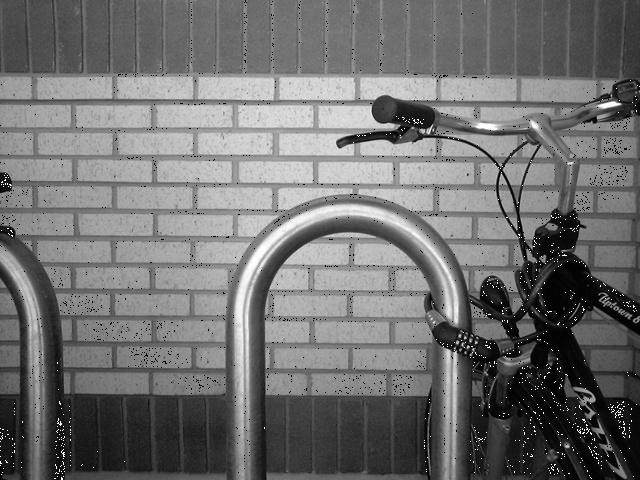
\includegraphics[width=\textwidth]{dst_sp.jpg}
        \caption{Figura com ruído sal e pimenta\cite{bike}}
        \label{fig:src_sp}
    \end{subfigure}
    \qquad
    \begin{subfigure}[ht]{0.4\textwidth}
        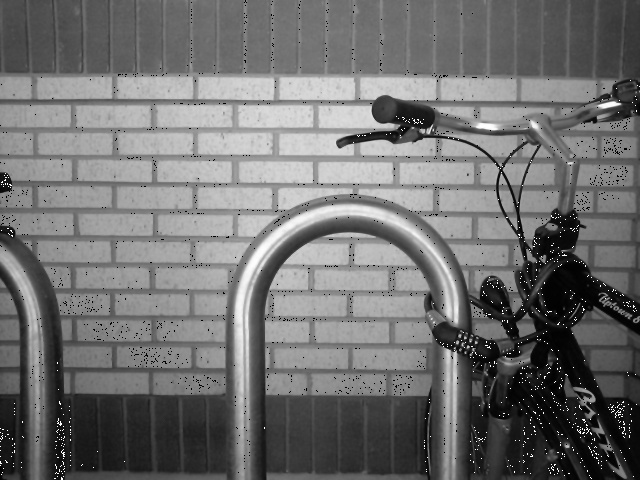
\includegraphics[width=\textwidth]{aniso_sp.jpg}
        \caption{\centering Após aplicação de difusão anisotrópica}
    \end{subfigure}
    \caption{Imagem com ruído sal e pimenta e com difusão anisotrópica}
    \label{fig:aniso_diff_sp}
\end{figure}

\subsection{Gaussiano}
Adicionando ruído do tipo gaussiano à imagem, obtemos o resultado expresso na Figura \ref{fig:aniso_diff_ga}.
\begin{figure}[!ht]
    \centering
    \begin{subfigure}[ht]{0.4\textwidth}
        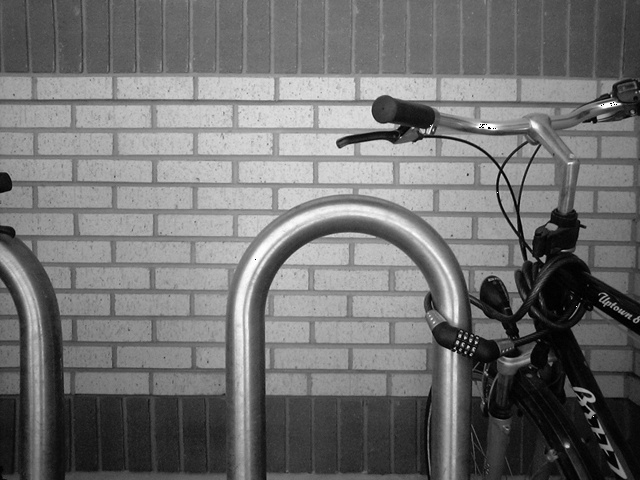
\includegraphics[width=\textwidth]{dst_ga.jpg}
        \caption{Figura com ruído gaussiano\cite{bike}}
        \label{fig:src_ga}
    \end{subfigure}
    \qquad
    \begin{subfigure}[ht]{0.4\textwidth}
        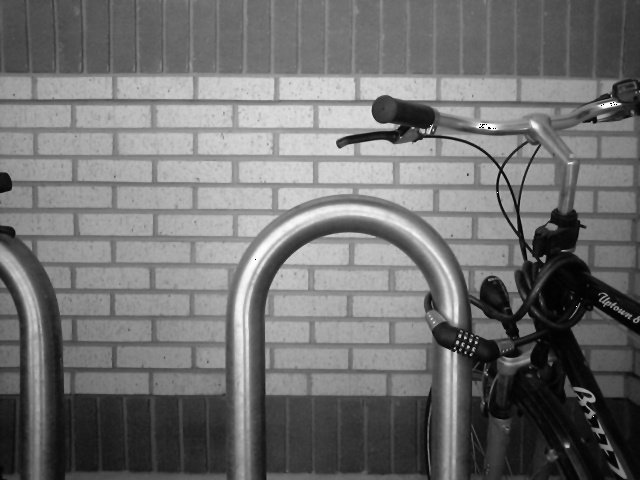
\includegraphics[width=\textwidth]{aniso_ga.jpg}
        \caption{\centering Após aplicação de difusão anisotrópica}
    \end{subfigure}
    \caption{Imagem com ruído gaussiano e com difusão anisotrópica}
    \label{fig:aniso_diff_ga}
\end{figure}

\section{Outros experimentos}
Realizou-se o experimento com outras imagens, como mostra a Figura \ref{fig:china}.
\begin{figure}[!ht]
    \centering
    \begin{subfigure}[ht]{0.4\textwidth}
        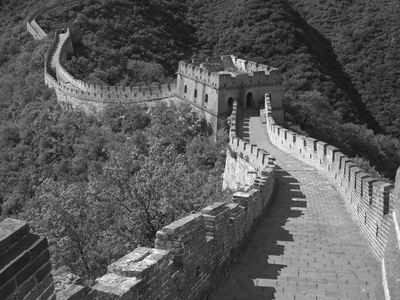
\includegraphics[width=\textwidth]{china_src.jpg}
        \caption{Figura original}
        \label{fig:china_src}
    \end{subfigure}
    \qquad
    \begin{subfigure}[ht]{0.4\textwidth}
        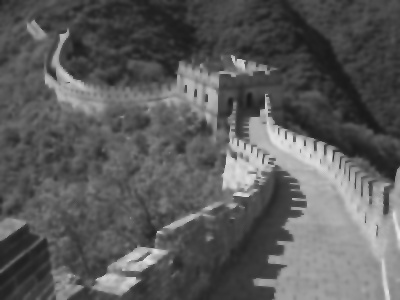
\includegraphics[width=\textwidth]{china_aniso.jpg}
        \caption{\centering Após aplicação de difusão anisotrópica}
        \label{fig:china_aniso}
    \end{subfigure}
    \\
    \begin{subfigure}[ht]{0.4\textwidth}
        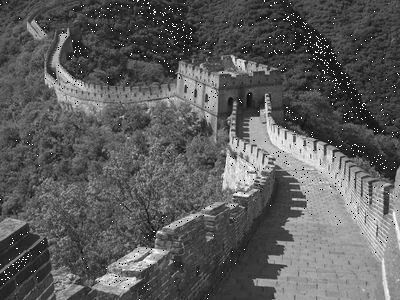
\includegraphics[width=\textwidth]{china_dst_sp.jpg}
        \caption{\centering Adição de ruído sal e pimenta}
        \label{fig:china_sp}
    \end{subfigure}
    \qquad
    \begin{subfigure}[ht]{0.4\textwidth}
        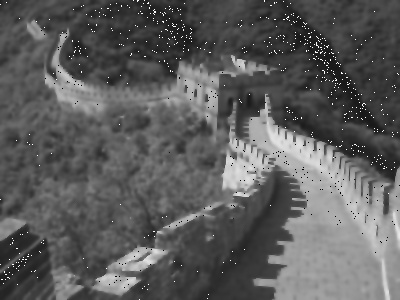
\includegraphics[width=\textwidth]{china_aniso_sp.jpg}
        \caption{\centering Após aplicação de difusão anisotrópica com ruído sal e pimenta}
        \label{fig:china_sp_aniso}
    \end{subfigure}
    \\
    \begin{subfigure}[ht]{0.4\textwidth}
        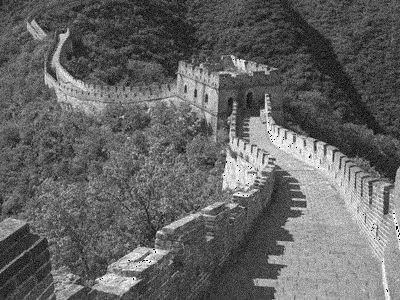
\includegraphics[width=\textwidth]{china_dst_ga.jpg}
        \caption{\centering Adição de ruído gaussiano}
        \label{fig:china_ga}
    \end{subfigure}
    \qquad
    \begin{subfigure}[ht]{0.4\textwidth}
        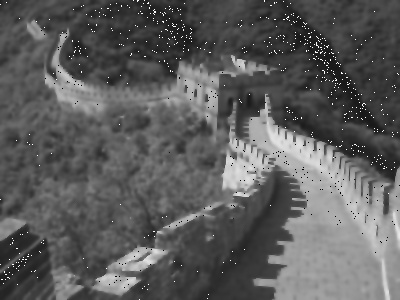
\includegraphics[width=\textwidth]{china_aniso_sp.jpg}
        \caption{\centering Após aplicação de difusão anisotrópica com gaussiano}
        \label{fig:china_ga_aniso}
    \end{subfigure}
    \caption{Aplicação de filtro anisotrópico em imagem com diferentes tipos de ruído.}
    \label{fig:china}
\end{figure}

\begin{thebibliography}{99}
    \bibitem{livro} GONZALEZ, Rafael C.; WOODS, Richard E.. \textbf{Digital Image Processing}. 3. ed. Upper Saddle River, NJ, EUA: Prentice-hall, 2006.
    \bibitem{opencv-sobel} \texttt{http://docs.opencv.org/doc/tutorials/imgproc/imgtrans/sobel\_derivatives/sobel\_derivatives.html}
    \bibitem{bike} \texttt{http://en.wikipedia.org/wiki/File:Bikesgray.jpg}
\end{thebibliography}

\end{document}
